\documentclass{article}
\usepackage[utf8]{inputenc}
\usepackage[T1]{fontenc}
\usepackage{graphicx}
\usepackage{amsmath, amssymb}
\usepackage{xcolor}
\usepackage{tikz}
\usepackage{enumitem}
\usepackage{lipsum}
\usetikzlibrary{fit}
\usepackage{hyperref} 
\usepackage{subfig}
\usepackage{polynom}
\usepackage{pgfplots}
\usepackage{soul}
\usepackage{framed}
\usepackage[most]{tcolorbox}

% Define colors
\definecolor{lessoncolor}{RGB}{74, 144, 226}
\definecolor{examplecolor}{RGB}{92, 184, 92}
\definecolor{notecolor}{RGB}{255, 179, 102}

\begin{document}

\begin{titlepage}
    \centering
    \vspace*{2cm}
    {\LARGE \textcolor{lessoncolor}{Advanced Functions}}\par
    \vspace{1cm}
    {\large Kensukeken}\par
    \vspace{2cm}
    {\large April 17th, 2024}\par
    \vspace{3cm}
\end{titlepage}
\tableofcontents
\newpage
\section{Unit 5}
\subsection{Graphing Trig Functions $\sin x$ \& $\csc x$ and $\cos x$ \& $\csc x$}
In this section, we will be relating the features of $\sin x$ and $\cos x$ to their reciprocals. You will notice that these reciprocals relate to the original function similar to linear reciprocals and quadratic reciprocals.

(insert table of values for $\sin x$ and $\csc x$)

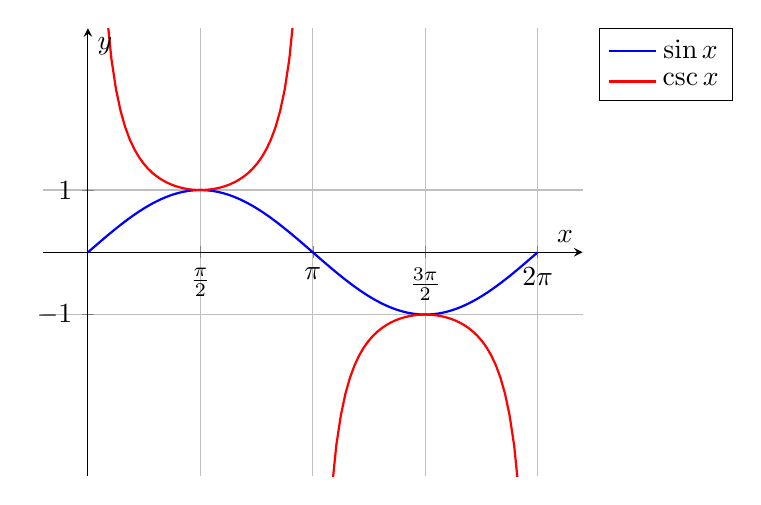
\begin{tikzpicture}
    \begin{axis}[
        domain=0:2*pi,
        samples=100,
        axis lines=middle,
        xlabel=$x$, ylabel=$y$,
        xtick={0, pi/2, pi, 3*pi/2, 2*pi},
        xticklabels={$0$, $\frac{\pi}{2}$, $\pi$, $\frac{3\pi}{2}$, $2\pi$},
        ytick={-1, 1},
        ymin=-3, ymax=3,
        grid=both,
        legend pos=outer north east,
        enlargelimits=true,
    ]
    \addplot [blue, thick] {sin(deg(x))};
    \addplot [red, thick, domain=0.01:pi-0.01, samples=50] {1/sin(deg(x))};
    \addplot [red, thick, domain=pi+0.01:2*pi-0.01, samples=50] {1/sin(deg(x))};
    \legend{$\sin x$, $\csc x$}
    \end{axis}
\end{tikzpicture}

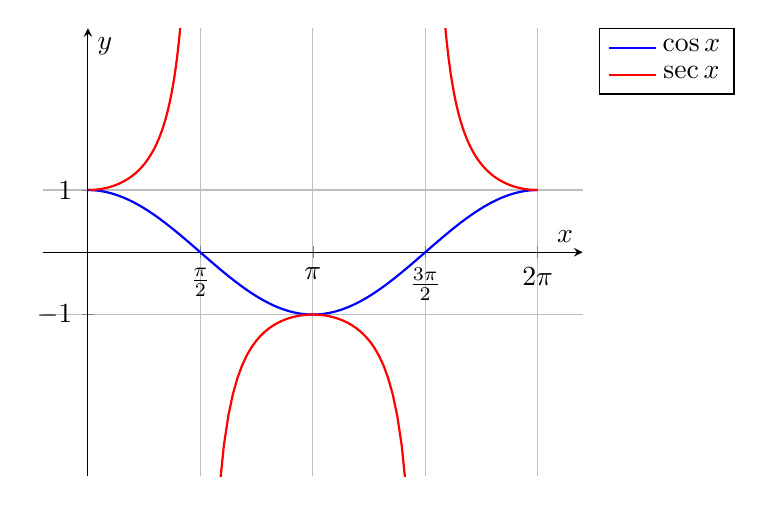
\begin{tikzpicture}
    \begin{axis}[
        domain=0:2*pi,
        samples=100,
        axis lines=middle,
        xlabel=$x$, ylabel=$y$,
        xtick={0, pi/2, pi, 3*pi/2, 2*pi},
        xticklabels={$0$, $\frac{\pi}{2}$, $\pi$, $\frac{3\pi}{2}$, $2\pi$},
        ytick={-1, 1},
        ymin=-3, ymax=3,
        grid=both,
        legend pos=outer north east,
        enlargelimits=true,
    ]
    \addplot [blue, thick] {cos(deg(x))};
    \addplot [red, thick, domain=0.01:pi/2-0.01, samples=50] {1/cos(deg(x))};
    \addplot [red, thick, domain=pi/2+0.01:3*pi/2-0.01, samples=50] {1/cos(deg(x))};
    \addplot [red, thick, domain=3*pi/2+0.01:2*pi-0.01, samples=50] {1/cos(deg(x))};
    \legend{$\cos x$, $\sec x$}
    \end{axis}
\end{tikzpicture}

Now, we will look at the key properties of the sine and cosecant functions.

\begin{tabular}{ |p{2cm}||p{5cm}|p{5cm}|  }
 \hline
 Property & $y = \sin x$ & $y = \csc x$\\
 \hline
 Period   & $2\pi$    & $2\pi$ \\
 \hline
 Max Value & 1 & N/A \textcolor{notecolor}{$\infty$ is NOT a value}\\
 \hline
 Min Value & -1 & N/A \textcolor{notecolor}{$\infty$ is NOT a value}\\
 \hline
 y-intercept & (0, 0) & N/A \\
 \hline
 x-intercept & 0, $\pi$, $2\pi$,... OR ($n\pi$, 0), $n\in \mathbb{Z}$(1)  & N/A\\
 \hline
 Vertical Asymptote & N/A & $x = n\pi, n\in \mathbb{Z}$ \textcolor{notecolor}{occurs at the x-int of $\sin x$}\\
 \hline
 Amplitude & 1 & N/A \textcolor{notecolor}{no max or min value}\\
 \hline
 Domain & $\{x\in \mathbb{R}\}$ & $\{x\in \mathbb{R}|x \neq n\pi, n\in \mathbb{Z} \}$\\
 \hline
 Range & $\{y\in \mathbb{R}|-1\leq y \leq 1\}$ & $\{y\in \mathbb{R}|y\leq -1, y \geq 1\}$\\
 \hline
\end{tabular}

\vspace{2em}

\section{Unit 5: Trig Functions \& Equations}
\textbf{Overview:} This unit consists of 5 video lessons. Allow no more than 12 class days for this unit, including time for review and to write the test.

\subsection{Graphs of Sine, Cosine and Tangent}
\[
\begin{array}{c}
y = \sin x \\
y = \cos x \\
y = \tan x \\
\end{array}
\]

\noindent Remember that \(\sin x\) is defined as the y-coordinate of the unit circle. This will be the distance above or below the x-axis.

\noindent For untransformed sinusoidal functions we have the following properties...

\subsubsection*{Example 1: Graph \( y = \sin x + 2 \)}
Vertical translation: now instead of oscillating around the x-axis, it will oscillate around the line \( y = 2 \).

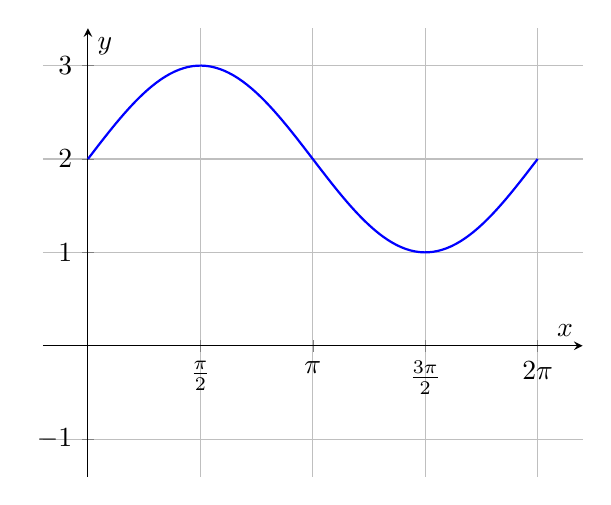
\begin{tikzpicture}
    \begin{axis}[
        domain=0:2*pi,
        samples=100,
        axis lines=middle,
        xlabel=$x$, ylabel=$y$,
        xtick={0, pi/2, pi, 3*pi/2, 2*pi},
        xticklabels={$0$, $\frac{\pi}{2}$, $\pi$, $\frac{3\pi}{2}$, $2\pi$},
        ytick={-1, 1, 2, 3},
        ymin=-1, ymax=3,
        grid=both,
        enlargelimits=true,
    ]
    \addplot [blue, thick] {sin(deg(x)) + 2};
    \end{axis}
\end{tikzpicture}

\subsubsection*{Example 2: Graph \( y = 2\cos x \) and \( y = -2\cos x \)}
Vertical stretch and reflection.

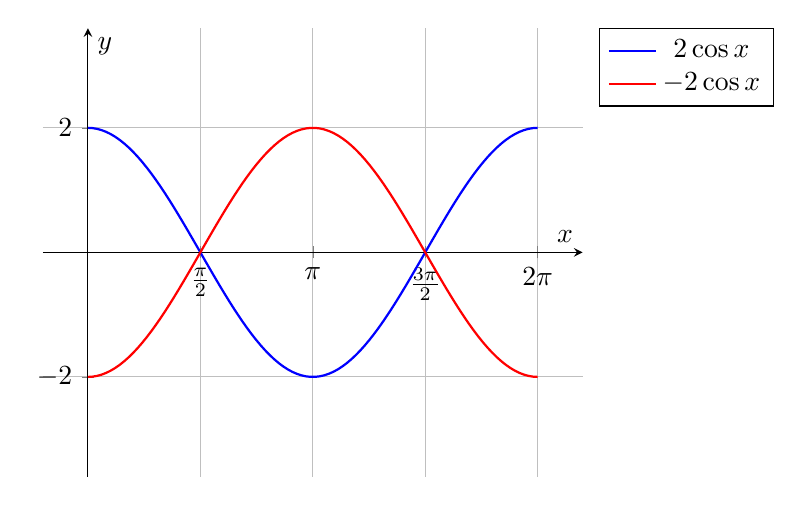
\begin{tikzpicture}
    \begin{axis}[
        domain=0:2*pi,
        samples=100,
        axis lines=middle,
        xlabel=$x$, ylabel=$y$,
        xtick={0, pi/2, pi, 3*pi/2, 2*pi},
        xticklabels={$0$, $\frac{\pi}{2}$, $\pi$, $\frac{3\pi}{2}$, $2\pi$},
        ytick={-2, 0, 2},
        ymin=-3, ymax=3,
        grid=both,
        legend pos=outer north east,
        enlargelimits=true,
    ]
    \addplot [blue, thick] {2*cos(deg(x))};
    \addplot [red, thick] {-2*cos(deg(x))};
    \legend{$2\cos x$, $-2\cos x$}
    \end{axis}
\end{tikzpicture}

\subsubsection*{Example 3: Graph \( y = \sin(x - \pi/2) \)}
Phase shift (horizontal translation) moves the function left or right.

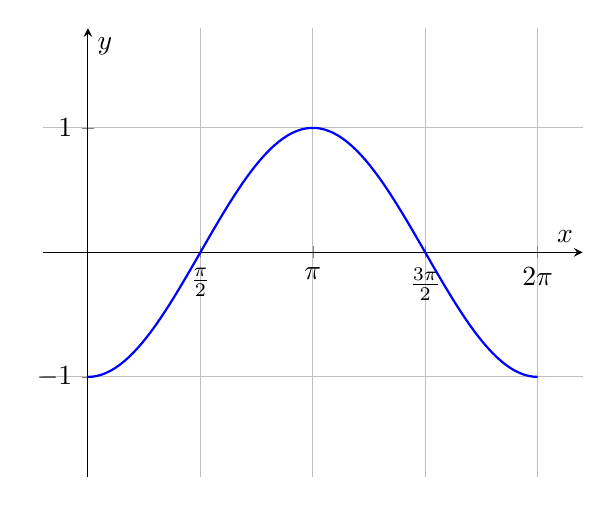
\begin{tikzpicture}
    \begin{axis}[
        domain=0:2*pi,
        samples=100,
        axis lines=middle,
        xlabel=$x$, ylabel=$y$,
        xtick={0, pi/2, pi, 3*pi/2, 2*pi},
        xticklabels={$0$, $\frac{\pi}{2}$, $\pi$, $\frac{3\pi}{2}$, $2\pi$},
        ytick={-1, 1},
        ymin=-1.5, ymax=1.5,
        grid=both,
        enlargelimits=true,
    ]
    \addplot [blue, thick] {sin(deg(x - pi/2))};
    \end{axis}
\end{tikzpicture}

\newpage

\subsection{Changing the Period}

\subsubsection*{Example 4: Graph the function \( y = \sin(3x) \)}
The 3 corresponds to a horizontal compression.

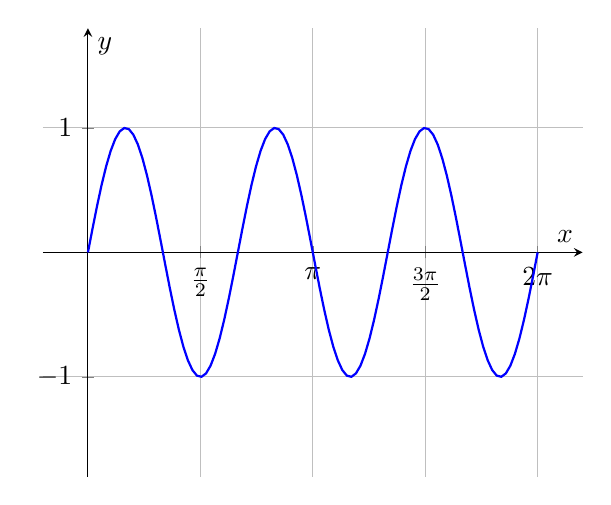
\begin{tikzpicture}
    \begin{axis}[
        domain=0:2*pi,
        samples=100,
        axis lines=middle,
        xlabel=$x$, ylabel=$y$,
        xtick={0, pi/2, pi, 3*pi/2, 2*pi},
        xticklabels={$0$, $\frac{\pi}{2}$, $\pi$, $\frac{3\pi}{2}$, $2\pi$},
        ytick={-1, 1},
        ymin=-1.5, ymax=1.5,
        grid=both,
        enlargelimits=true,
    ]
    \addplot [blue, thick] {sin(deg(3*x))};
    \end{axis}
\end{tikzpicture}

\subsubsection*{Example 5: Determine the value of \( k \) in \( y = \cos(kx) \) if the period is \( \pi/2 \)}

\[
\text{The period } T = \frac{2\pi}{k} = \frac{\pi}{2} \implies k = 4
\]

\newpage


\subsection{Reciprocal Trig Functions}
Complete the following graphs for \( y = \sec x \) and \( y = \cot x \).

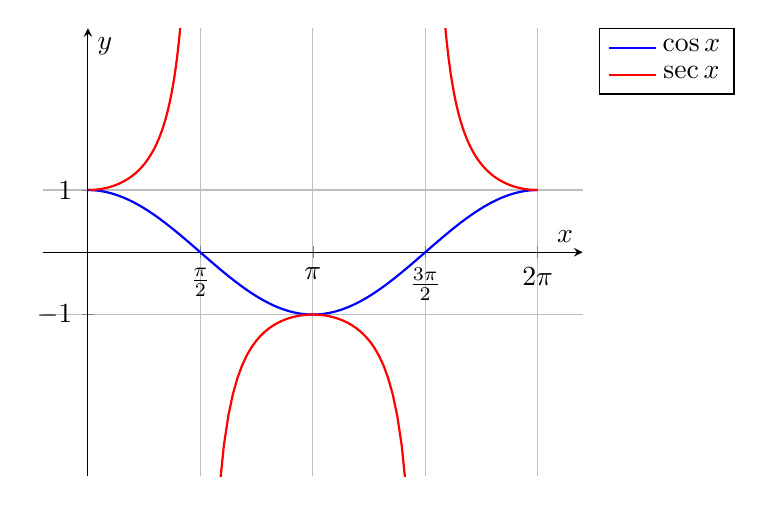
\begin{tikzpicture}
    \begin{axis}[
        domain=0:2*pi,
        samples=100,
        axis lines=middle,
        xlabel=$x$, ylabel=$y$,
        xtick={0, pi/2, pi, 3*pi/2, 2*pi},
        xticklabels={$0$, $\frac{\pi}{2}$, $\pi$, $\frac{3\pi}{2}$, $2\pi$},
        ytick={-1, 1},
        ymin=-3, ymax=3,
        grid=both,
        legend pos=outer north east,
        enlargelimits=true,
    ]
    \addplot [blue, thick] {cos(deg(x))};
    \addplot [red, thick, domain=0.01:pi/2-0.01, samples=50] {1/cos(deg(x))};
    \addplot [red, thick, domain=pi/2+0.01:3*pi/2-0.01, samples=50] {1/cos(deg(x))};
    \addplot [red, thick, domain=3*pi/2+0.01:2*pi-0.01, samples=50] {1/cos(deg(x))};
    \legend{$\cos x$, $\sec x$}
    \end{axis}
\end{tikzpicture}

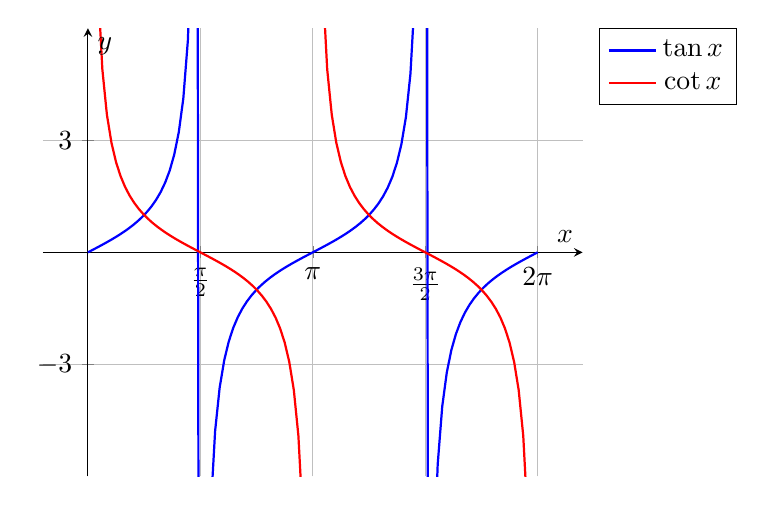
\begin{tikzpicture}
    \begin{axis}[
        domain=0:2*pi,
        samples=100,
        axis lines=middle,
        xlabel=$x$, ylabel=$y$,
        xtick={0, pi/2, pi, 3*pi/2, 2*pi},
        xticklabels={$0$, $\frac{\pi}{2}$, $\pi$, $\frac{3\pi}{2}$, $2\pi$},
        ytick={-3, 0, 3},
        ymin=-5, ymax=5,
        grid=both,
        legend pos=outer north east,
        enlargelimits=true,
    ]
    \addplot [blue, thick] {tan(deg(x))};
    \addplot [red, thick, domain=0.01:pi-0.01, samples=50] {1/tan(deg(x))};
    \addplot [red, thick, domain=pi+0.01:2*pi-0.01, samples=50] {1/tan(deg(x))};
    \legend{$\tan x$, $\cot x$}
    \end{axis}
\end{tikzpicture}

\newpage


\subsection{Sinusoidal Functions}
The general form of a sinusoidal function is:
\[
f(x) = a \sin [k (x - d)] + c
\]

\noindent Vertical Stretch: \( |a| > 1 \) \\
Vertical Compression: \( |a| < 1 \) \\
Reflection in x-axis: \( a < 0 \) \\
Horizontal Stretch: \( |k| < 1 \) \\
Horizontal Compression: \( |k| > 1 \) \\
Reflection in y-axis: \( k < 0 \) \\
Phase Shift: horizontal translation \\
Vertical translation: up \( c > 0 \), down \( c < 0 \)

\subsubsection*{Example 1: Graph \( y = 2\sin(\pi(x + 1)) - 3 \)}

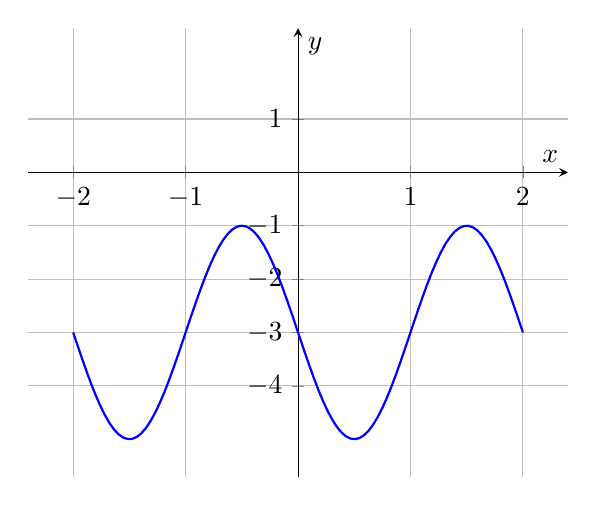
\begin{tikzpicture}
    \begin{axis}[
        domain=-2:2,
        samples=100,
        axis lines=middle,
        xlabel=$x$, ylabel=$y$,
        xtick={-2, -1, 0, 1, 2},
        ytick={-4, -3, -2, -1, 0, 1},
        ymin=-5, ymax=2,
        grid=both,
        enlargelimits=true,
    ]
    \addplot [blue, thick] {2*sin(deg(pi*(x + 1))) - 3};
    \end{axis}
\end{tikzpicture}

\subsubsection*{Example 2: Graph \( y = -5\cos(3x) + 1 \)}

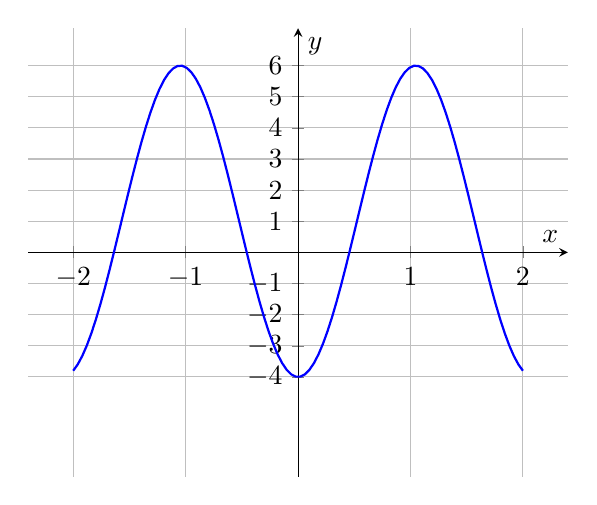
\begin{tikzpicture}
    \begin{axis}[
        domain=-2:2,
        samples=100,
        axis lines=middle,
        xlabel=$x$, ylabel=$y$,
        xtick={-2, -1, 0, 1, 2},
        ytick={-4, -3, -2, -1, 0, 1, 2, 3, 4, 5, 6},
        ymin=-6, ymax=6,
        grid=both,
        enlargelimits=true,
    ]
    \addplot [blue, thick] {-5*cos(deg(3*x)) + 1};
    \end{axis}
\end{tikzpicture}

\subsubsection*{Example 3: Find the form of the cosine curve that has an amplitude of 4, a period of \( 2\pi \), a left phase shift of \( \pi/4 \), and a vertical translation of 7.}

\[
y = 4\cos\left(x + \frac{\pi}{4}\right) + 7
\]

\subsubsection*{Example 4: Sketch the transformation of \( f(x) = \sin x \) with an amplitude of 3, period \( 2\pi \), and a phase shift of 0.5 radians to the right.}

\[
y = 3\sin\left(x - 0.5\right)
\]

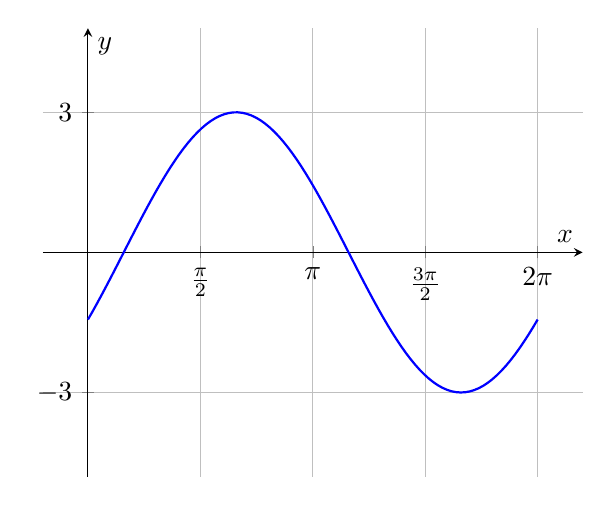
\begin{tikzpicture}
    \begin{axis}[
        domain=0:2*pi,
        samples=100,
        axis lines=middle,
        xlabel=$x$, ylabel=$y$,
        xtick={0, pi/2, pi, 3*pi/2, 2*pi},
        xticklabels={$0$, $\frac{\pi}{2}$, $\pi$, $\frac{3\pi}{2}$, $2\pi$},
        ytick={-3, 0, 3},
        ymin=-4, ymax=4,
        grid=both,
        enlargelimits=true,
    ]
    \addplot [blue, thick] {3*sin(deg(x - 0.5))};
    \end{axis}
\end{tikzpicture}

\newpage

\subsection{Solving Trigonometric Equations}

\subsubsection*{Example 1: Determine the solution to the equation \( 2\sin x + 1 = 0 \) for \( x \) in \([0, 2\pi]\)}

\[
2\sin x + 1 = 0 \implies \sin x = -\frac{1}{2}
\]
\[
x = \frac{7\pi}{6}, \frac{11\pi}{6}
\]

\subsubsection*{Example 2: Determine the solution to the equation \( 3(\tan x + 1) = 2 \) for \( x \) in \([0, 2\pi]\)}

\[
3(\tan x + 1) = 2 \implies \tan x = -\frac{1}{3}
\]
\[
x = \arctan\left(-\frac{1}{3}\right), \pi + \arctan\left(-\frac{1}{3}\right)
\]

\subsubsection*{Example 3: Determine the solution to the equation \( 2\sin^2 x - 3\sin x + 1 = 0 \) for \( x \) in \([0, 2\pi]\)}

\[
2\sin^2 x - 3\sin x + 1 = 0 \implies (2\sin x - 1)(\sin x - 1) = 0
\]
\[
\sin x = \frac{1}{2}, 1
\]
\[
x = \frac{\pi}{6}, \frac{5\pi}{6}, \frac{\pi}{2}
\]

\subsubsection*{Example 4: Determine the solution to the equation \( 2\sec^2 x - 3 + \tan x = 0 \) for \( x \) in \([0, 2\pi]\)}

\[
2\sec^2 x - 3 + \tan x = 0 \implies 2(1 + \tan^2 x) - 3 + \tan x = 0 \implies 2\tan^2 x + \tan x - 1 = 0
\]
\[
(2\tan x - 1)(\tan x + 1) = 0 \implies \tan x = \frac{1}{2}, -1
\]
\[
x = \arctan\left(\frac{1}{2}\right), \pi + \arctan\left(\frac{1}{2}\right), \arctan(-1), \pi + \arctan(-1)
\]

\subsubsection*{Example 5: Determine the solution to the equation \( 3\sin x + 3\cos^2 x = 2 \) for \( x \) in \([0, 2\pi]\)}

\[
3\sin x + 3\cos^2 x = 2 \implies 3\sin x + 3(1 - \sin^2 x) = 2 \implies 3\sin x + 3 - 3\sin^2 x = 2
\]
\[
-3\sin^2 x + 3\sin x + 1 = 0 \implies 3\sin^2 x - 3\sin x - 1 = 0
\]
\[
(3\sin x + 1)(\sin x - 1) = 0 \implies \sin x = -\frac{1}{3}, 1
\]
\[
x = \arctan(-\frac{1}{3}), \pi + \arctan(-\frac{1}{3}), \frac{\pi}{2}
\]

\newpage

\subsection{Making Connections to the "Real World"}

\subsection*{Making Connections}
We are going to use the graphing calculators for instantaneous rate of change.

\noindent On the graphing calculator:
\begin{itemize}
    \item Graph the curve \( y = \sin x \) (adjust your window so you see the curve better)
    \item Use the DRAW button \texttt{[2nd PRGM]} to draw on a tangent line
    \item Press \texttt{2nd PRGM}, choose 5: Tangent
    \item It will take you back to the graph, key in the x-value where you want the tangent line and press enter. Fill in the following table.
\end{itemize}

\noindent Many "real world" applications follow a cyclical or sinusoidal pattern. We can use a sinusoidal curve to model them. Usually we will choose the sine curve and apply a transformation to suit.

\subsubsection*{Example 1: The number of employees at a City Bicycle Company for each of the last 11 years is shown below. Find a sine curve that will model this data. Use technology to help you.}

\begin{minipage}{0.45\textwidth}
\begin{tabbing}
\hspace{1cm} \= \hspace{2cm} \= \kill
\textbf{Year} \hspace{1cm} \= \textbf{Employees} \\
1 \> 228 \\
2 \> 241 \\
3 \> 259 \\
4 \> 233 \\
5 \> 226 \\
6 \> 209 \\
7 \> 212 \\
8 \> 225 \\
9 \> 240 \\
10 \> 251 \\
11 \> 261 \\
\end{tabbing}
\end{minipage}

\begin{minipage}{0.45\textwidth}
\begin{align*}
\text{Amplitude (half the distance from max to min):} & \\
261 - 209 &= 52 \\
\frac{52}{2} &= 26 \\
\\
\text{Midline (the horizontal line right between max and min):} & \\
\frac{261 + 209}{2} &= 235 \\
\\
\text{Period (for k-value):} & \\
11 - 3 &= 8 \\
P = \frac{2\pi}{k} \implies 8 &= \frac{2\pi}{k} \\
8k &= 2\pi \\
k &= \frac{2\pi}{8} \implies k = \frac{\pi}{4} \\
\\
\text{Phase Shift (the x-value when the y is first on the midline):} & \\
& 1.3 \\
\end{align*}
\end{minipage}

\noindent The equation of the sine curve modeling the data is:
\[
y = 26\sin\left(\frac{\pi}{4}(x - 1.3)\right) + 235
\]

\end{document}
